\section{Consistency Check: $\Kstar$-Guided Filtering}
\label{sec:filtering}

$\Kempirical = 2$ makes a falsifiable prediction: binary curation should suffice, and graduated performance should converge toward binary as the decay steepness increases.
We present this as a consistency check under extreme contamination, not as an independent contribution; at realistic rates ($\leq$50\%), strategy differences remain below 0.3\,pp (Appendix~\ref{sec:dose_response}).
We compare six strategies on 30{,}000 documents (depths 0--5): (i)~\textbf{no-filter}, (ii)~\textbf{binary-ours} ($w = 1 - P(\text{synthetic})$ from 15D LightGBM), (iii)~\textbf{binary-Drayson}~\citep{drayson2025}, (iv)~\textbf{graduated} ($w = \exp(-\alpha \cdot \hat{d})$, $\alpha \in \{0.1,\ldots,0.9\}$), (v)~\textbf{surprisal} (retain above median), and (vi)~\textbf{DSIR}~\citep{xie2023dsir}.
We fine-tune Qwen2.5-1.5B-Instruct via Low-Rank Adaptation (LoRA; rank~8, $\alpha_{\text{LoRA}}{=}16$) for 3 epochs on MMLU and HellaSwag across 5 seeds (${\sim}$83\% synthetic; depth~0 retains human seeds~\cite{shumailov2024collapse, dohmatob2024model}).

\begin{table}[t]
\centering
\small
\caption{Downstream task performance (MMLU, HellaSwag) under six data-filtering strategies. Binary-ours uses the 15D LightGBM depth classifier; Graduated applies exponentially decaying weights $w = \exp(-\alpha \hat{d})$. Mean $\pm$ std over 5 seeds. Full $\alpha$ sweep in Figure~\ref{fig:filtering_strategies}.}
\label{tab:tab_filtering_main}
\resizebox{\columnwidth}{!}{\begin{tabular}{lcc}
\toprule
\textbf{Strategy} & \textbf{MMLU} & \textbf{HellaSwag} \\
\midrule
Base model (no training) & 0.6018 & 0.6821 \\
\midrule
Binary-ours ($\Kstar{=}2$) & \textbf{0.5941}$\pm$0.0008 & \textbf{0.6701}$\pm$0.0006 \\
Binary-Drayson & 0.5913$\pm$0.0009 & 0.6691$\pm$0.0004 \\
Surprisal & 0.5894$\pm$0.0009 & 0.6641$\pm$0.0006 \\
Graduated ($\alpha{=}0.9$) & 0.5892$\pm$0.0008 & 0.6701$\pm$0.0007 \\
DSIR & 0.5869$\pm$0.0003 & 0.6631$\pm$0.0007 \\
No filter & 0.5865$\pm$0.0010 & 0.6638$\pm$0.0008 \\
\bottomrule
\end{tabular}
}
\end{table}

\begin{figure}[t]
\centering
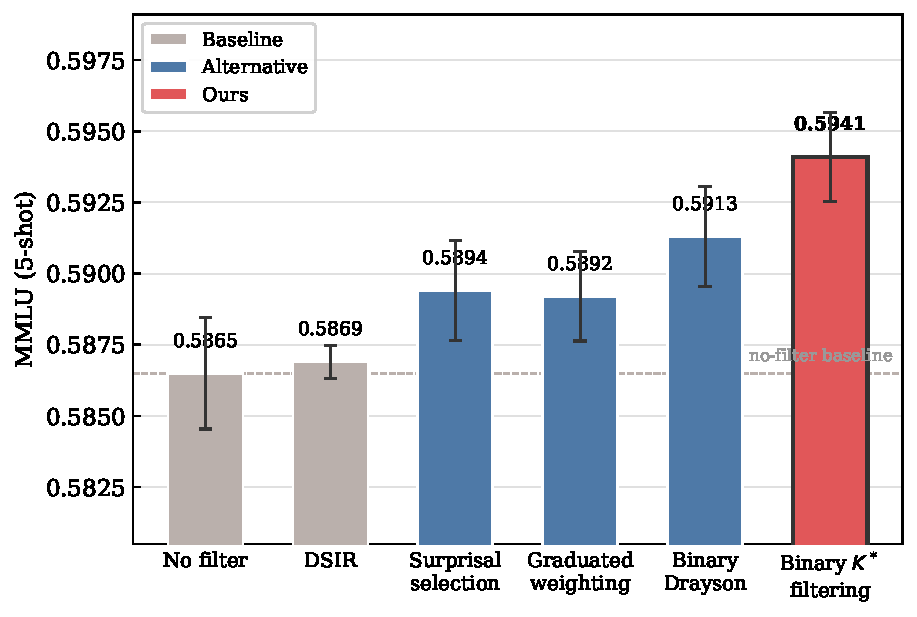
\includegraphics[width=\columnwidth]{figures/fig_filtering_strategies.pdf}
\caption{MMLU accuracy under six filtering strategies (5 seeds, $\pm$1 std). Binary $\Kstar$ filtering (red) minimizes degradation; graduated weighting converges toward binary as $\alpha$ increases. Dashed line: no-filter baseline.}
\label{fig:filtering_strategies}
\end{figure}

Binary-ours reduces the MMLU gap from $-$1.53\,pp (no-filter) to $-$0.77\,pp (${\sim}$50\% reduction; $p_{\text{corr}} < 0.05$ vs.\ all alternatives; Table~\ref{tab:tab_filtering_main}, \ref{tab:pairwise_significance}).
The ordering is interpretable through $\Kempirical$: binary filtering exploits the strongest boundary (0v1), while graduated strategies assign weights based on near-random classifier outputs, injecting noise.
Graduated filtering converges toward binary: at $\alpha{=}0.9$, it matches binary-ours on HellaSwag ($p_{\text{corr}} = 1.00$) but remains worse on MMLU ($p_{\text{corr}} = 0.011$); DSIR is indistinguishable from no-filter (Figure~\ref{fig:filtering_strategies}).
At realistic contamination ratios ($\leq$50\%), strategy differences remain below 0.3\,pp (Appendix~\ref{sec:dose_response}); this extreme setting validates $\Kempirical$'s predictive power despite vanishing effect sizes at realistic ratios.
